\documentclass{article}
\usepackage[utf8]{inputenc}
\usepackage{graphicx}
\usepackage{subfigure}
\usepackage{multicol}
\usepackage{lipsum}
\usepackage{mwe}
\oddsidemargin -0.04cm   
\evensidemargin -0.04cm
\textwidth 16.59cm
\textheight 22.94cm 

\title{Hysteranthy variability II}
\author{Daniel Buonaiuto, Nacho, Lizzie}
\date{December 2018}

\begin{document}

\maketitle

\section{Introduction}

\begin{enumerate}
    \item Phenological sequences are important % define hysteranthy seranthy and synanthy
    \begin{enumerate}
        \item FLS has received attention.
        \item While in typical plant models, vegetative growth proceeds reproduction, hysteranthy, flowering first, is extremely common in the temperate zone.
        \item This begs the question is there some adaptive significance? In fact, several hypotheses have been proposed:
    \end{enumerate}
    \item Hypotheses
    \begin{enumerate}
        \item Wind pollination
        \item Water dynamics
        \item Early flowering
        \item Phylogenetic constraint
    \end{enumerate}
    \item While advances have been made in characterizing FLS (Gougherty), our understanding of this traits remains in its infancy. 
    \begin{enumerate}
        \item This is alarming, because as we can see in Figure 1, hysteranthy is changing.

     \item As can be seen in figure 1, the the FLS response to climate change differs between species. All species increase their offset, but the rate of change differs between species. In fact, the mean FLS offset for one species, \textit{Fraxinus excelsior} has already exceeded its historic range of variability, while \textit{Aesculus hippocastanum} FLS shows a more muted response. Depending on the function of FLS, this differential FLS sensitivity to climate change may have implications for community composition and population demography in the future.
    \end{enumerate}
    \item As the study of phenology has matured as a discipline, it has become clear measure of synchrony and variability are a key part of the adaptive significance of phenology, and we expect that this would hold true for phenological sequences as well.
    \begin{enumerate}
        \item However, while some have found general correlation between flowering leafing (\citep{Lechowicz}), fine scale FLS variability has never been evaluated.
        \item We suggest that characterizing FLS variation among individuals, populations and over time, will allow for a more biologically relevant evaluation of the current FLS hypotheses as well as reveal avenues for future direct hypothesis testing.
    \end{enumerate}
\item We will discuss  1) how variability would affect our conception of the FLS hypotheses, 2) evidence for the scope of FLS variability in existing data, 3) Models, 4) recommendations for further FLS study.
\end{enumerate}

\section{Variability and the Characterization of FLS}
\begin{enumerate}
\item There are two type of data that can be used to evaluate FLS: Qualitative, categorical descriptions of FLS from regional guidebooks or flora, or quantitative observations of leaf and flower phenology from long term data sets or experiments. The advantage of categorical datasets are that they include a much wider taxonomic range, while quantitative observations are restricted to a limited number of species and locations.  However, all categorical characterizations are based on empirical observations, and this conversion from quantitative to qualitative structure comes with cost that we will demonstrate below.
\begin{enumerate}
    \item First let us consider how we might characterize the FLS's of the 6 species in figure \ref{fig:Figure 2} based on their species level averages over the 15 year observation periods. 
    \begin{enumerate}
    \item \textit{Acer rubrum} opens its flower buds and flowers, before leaf budburst and leaf expansion. This species' FLS would clearly be classified as hysteranthous.
    \item  The opposite is true for \textit{Nyssa sylvactica}, which would clearly be classified as seranthous as its flower bud burst and flower opening occur after leaf expansion.
    \item But what about less straight forward cases like \textit{Betula allaghaniensis}? One would be justified in classifying the species as hysteranthous for its flower buds bursting before its leaf buds, or as synanthous for the fact the its open flowers overlap its leaf budburst and development. Can we really put this species in the same category as \textit{Acer rubrum}, whose flowers open weeks before the leaves? Conversely, is this species truly similar to \textit{Acer pensylvanicum} whose flowers, while overlapping leaf growth, do not open until leaves are well along in their expansion? It is clear that either choice will obscure important interspecific differences between the species in the community.
    \end{enumerate}
 \item This ambiguity discussed above, is not just a exercises in trivial categorization, but matters to how we think about FLS hypothesis testing.
 \begin{enumerate}
     \item For example, the wind pollination hypothesis suggests that hysteranthous flowering is an adaptation for wind pollination, and as such, would be more likely to be associated with this syndrome. While, according to figure \ref{fig:Figure 1}, a species like \textit{Fraxinus americana} would be most accurately categorized as synanthous is it a reasonable to assert that pollen transfer would be so adversely affected by developing leaves that only burst a day or two prior to flower viability? All four of the "synanthous" species flower weeks ahead of the time their leaves reach 75\% of their full size. It would be fair to argue that this FLS offset could be equally adaptive for wind pollination as the clear hysteranthy of \textit{Acer rubrum}.
     \item However, if we were to consider the water stress hypothesis, we expect that any period in which leaf tissue was transpiring would compromise flowering, we would expect, and this hypothesis would suggest that \textit{Acer rubrum} alone, and perhaps \textit{Betula alleghaniensis} are adapted.
 \end{enumerate}
  \item It is clear, that this categorical system muddies our ability to test trait hypotheses. We will discuss how this ambiguity can be account for in part 3, when we lay out a framework for modeling trait association. 
  \end{enumerate}
    
 \item Broad FLS characterization not only masks potentially important interspecific differences, it also masks other kinds of  variability, whose elucidation would be useful for FLS hypothesis testing.
        \item Consider, for example, the annual FLS of the \textit{Quercus rubra} community at Harvard forest in \ref{fig:Figure 3} and the following trend become apparent.
        
        \begin{enumerate}
        \item  This is a species classically listed as synanthous, and our average values would agree.
        \item But in fact, there are some years in which flower bud bust is over a week before leaf bud burst, and other years, in which leaf buds burst weeks prior to floral bud bust.
        \item Additionally, while the overall trends in phenology are the same for all three individuals observed, their degree of FLS offset can differ significant within years and there are year where their FLS do not match (2005, 2007).
    \end{enumerate}
 
    \item Accounting for this variability could be a valuable for hypothesis testing.
    \begin{enumerate}
        \item With this kind of data we could ask:
        \item Do years of drought stress increase dissociation between flowering and leaves? Do wetter areas have less offset?
        \item Do increase offset years result in more pollination success or increased reproductive output?
        \item Do areas will less risk of late season frost have less FLS offset? 
    \end{enumerate} %%% should I actually test this? See section 3.4

\item Over all we see, variation is significant. This variation should be accounted for. can be done most effectively with quantitative data, but greater effort could be made to incorporate variability into categorical data too, which we will discuss below.
\end{enumerate}

\section{Hypothesis testing}
\begin{enumerate}
    \item Considering qualitative data:
    \begin{enumerate}
    \item The basic framework evaluating the strength of the hypotheses is to model the association between FLS and predictors that reflect the basic hypotheses. We obtained FLS data from two sources, Michigan Trees Shrubs and Vines and USFS Silvics Manual Vol II. From these sources, we obtained trait data on pollination syndrome and average flowering month. For each species, we also obtained the minimum precipitation tolerated across the species's range from the USDA's conservation plant database. These categorical response variables are most easily interpreted in the model when collapsed to binary.  Applying different binning schemes elucidates the interspecific variability in FLS, and clarifies the hypotheses. 
       \item We binned hysteranthy in two different ways: physiological (only ``flowers before leaves") and functional (``flowers before leaves" and ``flowers before/with leaves", and ``flowers with leaves") for both data sets. 
    \item As can be seen in the figure: 
    \begin{enumerate}
        \item  Early flowering predicts hysteranthous FLS regardless of the classification scheme. We found that this relationship was maintained even win the data was subset to only species that flowered before mid-May.
        \item We see that pollination syndrome is a strong predictor of hysteranthous FLS for the functionally defined hysteranthy. This fits with our biological assertion that wind pollination efficiency is maintained as long as flowers are open during the early stages of leaf expansion.
        \item In out model we see no effect of minimum precipitation for any of the classification. This makes sense, because precipitation is probably not limiting in the spring, so there would be no selection for hysteranthy. But it contradicts recently modeling studies \citep{Gougherty2018}.
        \item For functional hysteranthy, there is a interaction between pollination syndrome and minimum precipitation,  as well as flowering time and minimum precipitation.
        \item  increases p min (less drought tolerant) decreases the negative association with flowering time. So more drought tolerance and earlier are increase the likelihood of hysteranthy
        \item increased p min (less tolerance) increases the positive association with wind pollination. hysteranthous insect pollinated species are more likely to be drought tolerant. This makes sense with the fact the this hypothesis is tropical in origin.
        \item The phylogenetic signal also varies with these choices.\\ 
        \begin{tabular}{|c|c|}
           \hline
            Hysteranthy class & D statistics \\
            \hline
             Functional MTSV & 0.06\\
             Physiological MTSV & 0.29\\
             Functional USFS & 0.65\\
             Physiological USFS & 0.11\\ % how do I interpret this should talk to Jonathan and make him author?
             \hline
        \end{tabular}
    \end{enumerate}
   \item While we can make some nuanced inference with this scheme, we are still limited by categorical data. Treating FLS as continuous is more biological accurate and allows for stronger inference. 
    \end{enumerate}
    \item We illustrate this by running a similar model with FLS treated as a continuous predictor base on phenological data collected at Harvard forest. We approximate the functional/physiological hysteranthy classification by treating the offset between flower and leaf budburst as physiological hysteranthy and the offset between flowers opening and leaves reaching 75\% of their final size as functional hysteranthy.
    \begin{enumerate}
        \item We seeing Figure 5a That flowering day is still the strongest predictor. 
        \item We see also that for both classification schemes pollination syndrome is also important.
        \item there is no effect of min P.
        \item When we convert these data to binary in figure 6b, we similar overall patterns pattern, but the, but the agreement between the classification schemes effect sizes and confidence change dramatically. % how much to talk about the interactions? Should we even include them
    \end{enumerate}
    \item Synthesis: Flowering time always important. Pollination syndrome tends to matter. Min precip seems not to matter much but, it is not necessarily a great predictor of drought tolerance. 
    
    \item PEP site or HF interannual variation with climatological data %I could do this
    \begin{enumerate}
    \item offset~ average precept, or average date of last frost
    \item expectation less offset= earler last frost= higher precip
    \item or one site by year. could do this at HF too
    
    \end{enumerate}
    \end{enumerate}
 \section{Moving forward}
 \begin{enumerate}
     \item Continuous data should be a priority
     \item tease out biogeographic elements of this question
     \item What is the mechanism?
     \item direct test of fitness
 \end{enumerate}

\begin{figure}
    \centering
 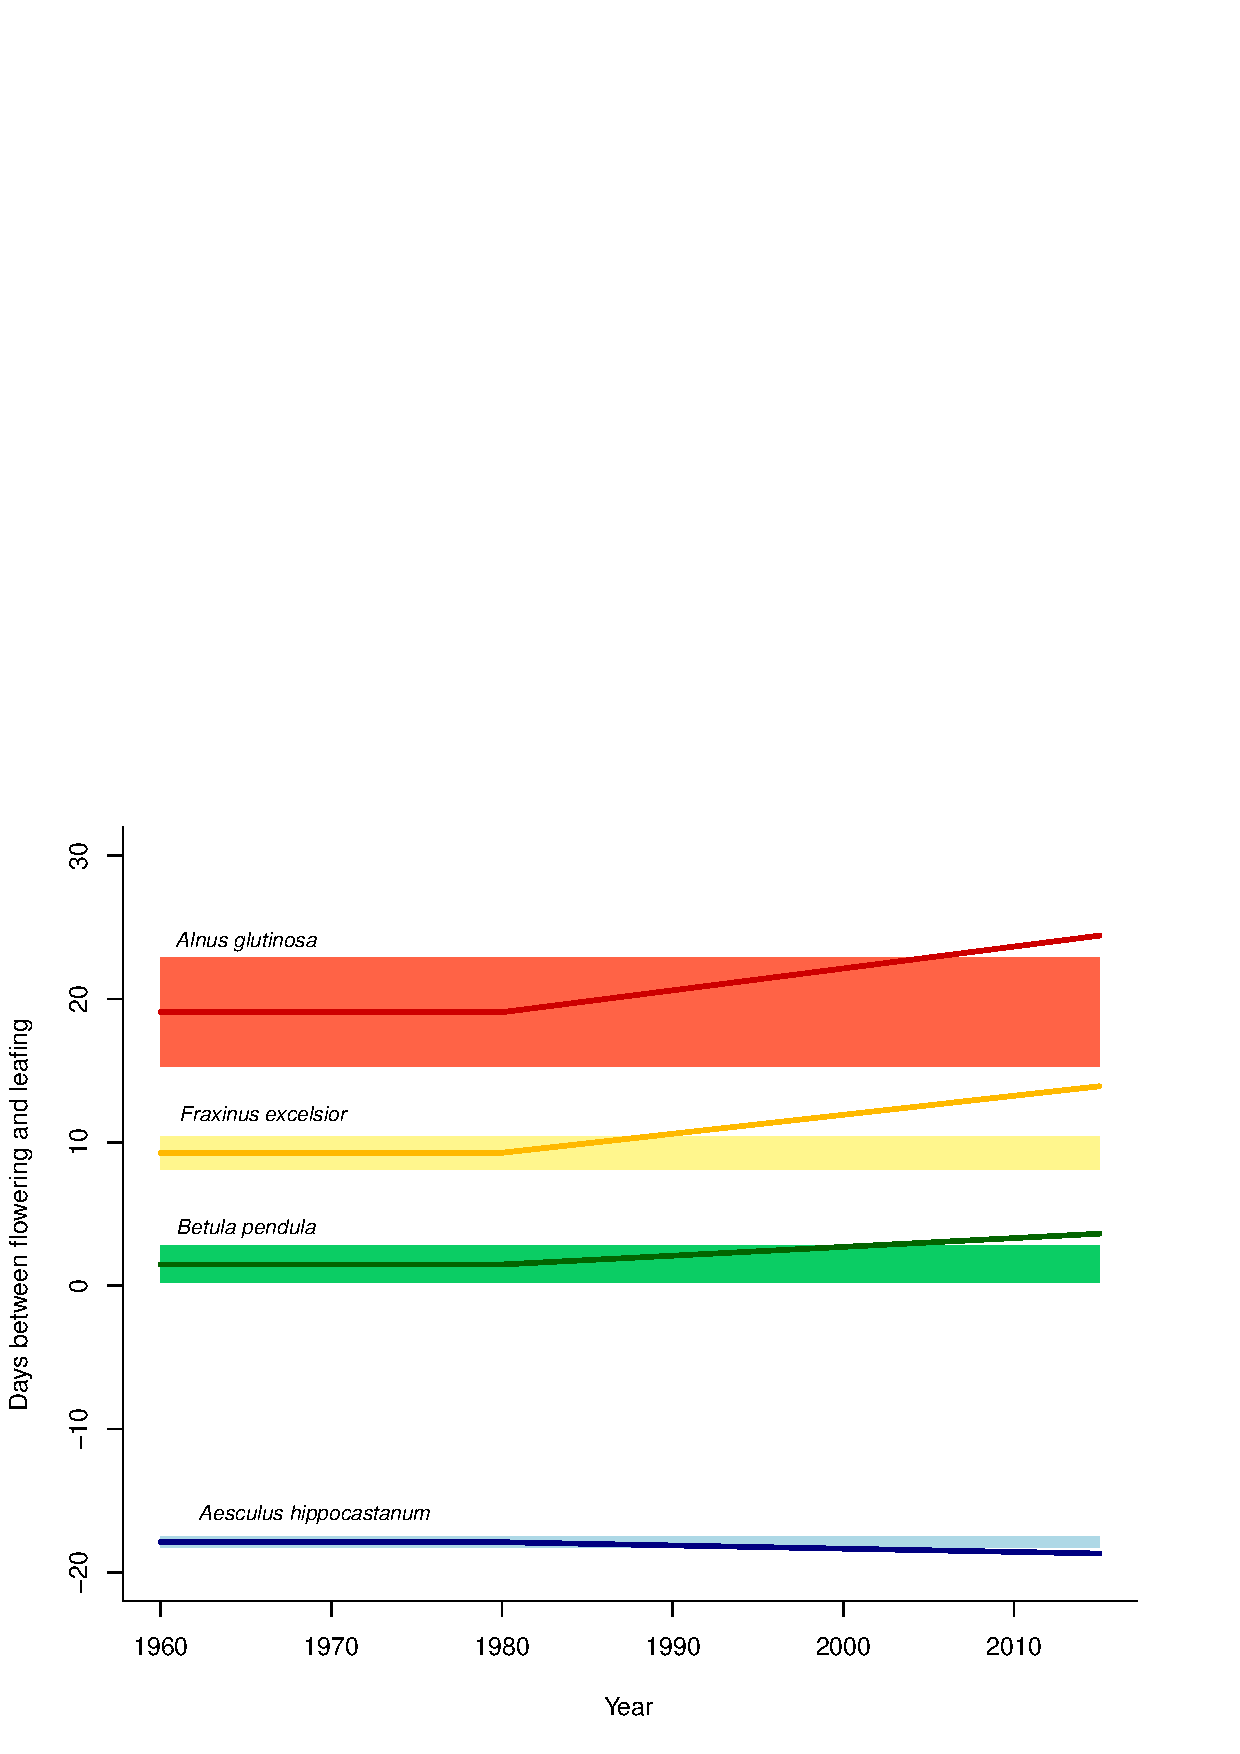
\includegraphics[width=\textwidth]{FLS_climate_change.jpeg} 
    \caption{Trends in average FLS offset across Europe for 3 tree species from 1960 to 2015. Dashed lines indicate historic range of FLS variability. All species are increasing their offset, but the rate of change differs between species and and sites}
    \label{fig:Figure 1}
\end{figure}
\begin{figure}
    \centering
    \includegraphics[width=\textwidth]{HFmeans.jpeg}
    \caption{Average day of phenological events for six woody plant species at Havard Forest in Petersham, MA from 1990-2015}
    \label{fig:Figure 2}
\end{figure}
 \begin{figure}
        \centering
          \includegraphics[width=\textwidth]{HF_dissplot.pdf}
        \caption{FLS variability among years and within a population of \textit{Quercus rubra} at Harvard forest.}
        \label{fig: Figure 3}
    \end{figure}
     \begin{figure}
    \centering
    \includegraphics[width=\textwidth]{MTSV_USFS_compsplots.jpeg}
    \caption{Currently only showing MTSV results}
    \label{fig:Figure 4}
\end{figure}
    \begin{figure}
    \centering
    \includegraphics[width=\textwidth]{HF_bin_v_cont_effectsizes.jpeg} 
    \caption{Effect sizes of predictors in HF}
    \label{fig:Figure 5}
    \end{figure}



    \begin{figure}
    \centering
    \includegraphics[width=\textwidth]{MTSV_USFS_compsplots_noint.jpeg} 
    \caption{Same as plot 4 with noint}
    \label{fig:Figure 6}
    \end{figure}
    
        \begin{figure}
    \centering
    \includegraphics[width=\textwidth]{HF_noint_bin_v_cont_effectsizes.jpeg}
    \caption{same as fig 5 with no in}
    \label{fig:Figure 7}
    \end{figure}



\end{document}
